% 原书 p.299–p.302（PDF p.307–p.310）；第 10 章 10.3 节（层上同调）
% 说明：本文件不含 \chapter（第 10 章标题由 ch10a-s01 写出）。PDF p.307 顶部仍是 10.2 节
%       的收尾（图 10.3、承接 p306 末句的段落与注 10.2.5），按页范围由本文件承接，
%       之后才是 10.3 节。
% >>> p307
\begin{figure}[htbp]
  \centering
  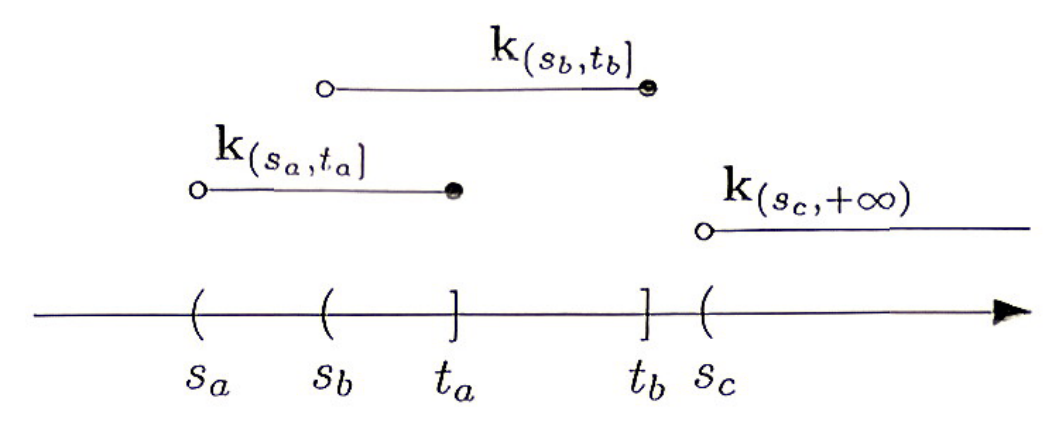
\includegraphics[width=0.72\linewidth]{figures/fig_p307_1.png}
  \caption*{图 10.3\quad $\R_\gamma$ 上的可构造层（原书 p.299, Figure 10.3；
  PDF p.307）}
\end{figure}

探讨这两族 $\mathbf{k}_I$ 之间的关系，是一个有趣的问题（cf.\ [246] 的附录 A）。

% [Tutor Note: 记号依据——上一页（PDF p306）把定理 10.2.1 与定理 5.2.1 中的「积木」
% $\mathbf{k}_I$ 作了比较：前者是 $\R_\gamma$ 上关于局部闭子集 $I$ 裁剪的常值层，
% 后者是区间型持续模。图 10.3 画出的是层版本：水平轴为 $\R_\gamma$ 的「时间」轴，
% 每条水平线段表示一个区间 $I=(s,t]$ 上的常值层 $\mathbf{k}_I$（左端开、右端闭），
% 三条线段 $I=(s_a,t_a]$、$(s_b,t_b]$、$(s_c,+\infty)$ 给出分解中的三个直和项。
% 注意 $t=+\infty$ 的区间在图中画成向右无限延伸。]

\begin{wrem}{10.2.5}
回忆：对一个持续 $\mathbf{k}$-模 $\mathbb V$，它所含的信息不止是各纤维的维数。事实上，
$\mathbb V$ 的理论深度来自结构映射 $\iota_{s,t}:V_s\to V_t$（$s\leqslant t$）。类似地，
由定理 10.2.1，读出可构造层 $\mathcal F\in\mathrm{Ob}(\operatorname{Sh}(\mathbf{k}_{\R_\gamma}))$
的各茎是相当容易的，而另一个关键信息来自两个茎之间的关系。确实，对任意
$s\leqslant t$，层的公理性质蕴涵：对任意 $s\leqslant t$，存在从茎 $\mathcal F_s$ 到
$\mathcal F_t$ 的 $\mathbf{k}$-线性映射。确切地说，按定义
\[
\mathcal F_s=\varinjlim_{\varepsilon\to0}\mathcal F\bigl((s-\varepsilon,\infty)\bigr)
\xrightarrow{\operatorname{res}_{s,t}}
\varinjlim_{\varepsilon\to0}\mathcal F\bigl((t-\varepsilon,\infty)\bigr)=\mathcal F_t,
\]
其中映射 $\operatorname{res}_{s,t}$ 是由限制映射
$\mathcal F((s-\varepsilon,\infty))\to\mathcal F((t-\varepsilon,\infty))$、连同正向极限
的泛性质所诱导的映射（见练习 10.2.3）。
\end{wrem}

% [Tutor Note: 易错预警——注 10.2.5 中 $\operatorname{res}_{s,t}$ 的方向容易与限制映射
% 混淆：$\mathcal F_s$ 是 $(s-\varepsilon,\infty)$ 上的截面在 $\varepsilon\to0$ 时的正向
% 极限，而 $(s-\varepsilon,\infty)\supset(t-\varepsilon,\infty)$（当 $s\leqslant t$），
% 故限制映射的方向是 $\mathcal F((s-\varepsilon,\infty))\to\mathcal F((t-\varepsilon,\infty))$，
% 与 $\operatorname{res}_{s,t}$ 一致。这一族映射正是持续模的结构映射 $\iota_{s,t}$ 的
% 层论版本；定理 10.2.1 的分解把「茎」与「茎间关系」分开处理，正是持续模理论的层论
% 对应物。]

\section{层上同调（Sheaf Cohomology）}

\begin{keytakeaways}
\begin{itemize}
  \item 几何图像：层上同调同时测量空间 $X$ 的拓扑与 $X$ 上（$\mathbf{k}$-模）层
        $\mathcal F$ 的「扭曲」；Čech 上同调用开覆盖的交叠截面把局部数据组织成上链
        复形，其障碍在于交叠处截面的相容性。
  \item 数学工具：开覆盖 $\{U_i\}_{i\in I}$ 上的 Čech 复形
        $C^n=\prod_{i_0<\cdots<i_n}\mathcal F(U_{i_0\cdots i_n})$，微分由 (10.14)
        给出；上同调群 (10.15) 为 $\ker/\operatorname{im}$；再对覆盖的加细取正向极限
        得到 $H^*(X;\mathcal F)$（定义 10.3.1）。
  \item 本节结论：Leray 定理——若覆盖满足无环条件 (10.16)，则 Čech 上同调直接等于
        $H^*(X;\mathcal F)$；例 10.3.2 用它算得 $H^*(\R;\mathbf{k}_{(0,1]})=0$。
  \item 遗留问题：层上同调群究竟度量 $X$ 的复杂度还是层 $\mathcal F$ 的复杂度
        （问题 10.3.1）？这需要 10.4 节引入的导出函子视角来回答。
\end{itemize}
\end{keytakeaways}

层上同调理论是一种同时研究空间 $X$ 的拓扑与 $X$ 上（$\mathbf{k}$-模）层
$\mathcal F$ 的上同调方法。它有多个版本，我们将从最具可计算性的一个——\textbf{Čech
上同调}——开始。

设 $X$ 是流形，$\{U_i\}_{i\in I}$ 是 $X$ 的开覆盖。对任意一族两两不同的指标
$(i_0,\cdots,i_n)\subset I$，引入记号
$U_{i_0\cdots i_n}:=U_{i_0}\cap\cdots\cap U_{i_n}$，并构造一个上链复形，其次数为 $n$
的部分是如下 $\mathbf{k}$-模
\begin{equation}\tag{10.13}
C^n(\{U_i\}_{i\in I};\mathcal F):=
\prod_{i_0<\cdots<i_n}\mathcal F(U_{i_0\cdots i_n})
=\prod_{i_0<\cdots<i_n}\mathcal F(U_{i_0}\cap\cdots\cap U_{i_n}).
\end{equation}
特别地，$C^0(\{U_i\}_{i\in I};\mathcal F)=\prod_{i\in I}\mathcal F(U_i)$。所需的
微分 $\dd^n:C^n(\{U_i\};\mathcal F)\to C^{n+1}(\{U_i\};\mathcal F)$ 定义如下：对截面
$s\in C^n(\{U_i\};\mathcal F)$，按定义
$\dd^n s\in C^{n+1}(\{U_i\}_{i\in I};\mathcal F)$，其每个分量由下式给出
% >>> p308
\begin{equation}\tag{10.14}
(\dd^n s)_{i_0\cdots i_{n+1}}:=
\sum_{k=0}^{n+1}(-1)^k
s_{i_0\cdots\widehat{i_k}\cdots i_{n+1}}\big|_{U_{i_0\cdots i_{n+1}}}
\in\mathcal F(U_{i_0\cdots i_{n+1}}),
\end{equation}
其中
$s_{i_0\cdots\widehat{i_k}\cdots i_{n+1}}|_{U_{i_0\cdots i_{n+1}}}$ 表示
$s_{i_0\cdots\widehat{i_k}\cdots i_{n+1}}$ 在限制映射
$\operatorname{res}:\mathcal F(U_{i_0\cdots\widehat{i_k}\cdots i_{n+1}})
\to\mathcal F(U_{i_0\cdots i_{n+1}})$ 下的像。

% [Tutor Note: 易错预警——(10.14) 中有三处容易抄错：(i) 求和中 $\widehat{i_k}$ 表示
% \emph{删去}指标 $i_k$；(ii) 符号是 $(-1)^k$，求和从 $k=0$ 到 $n+1$，共 $n+2$ 项；
% (iii) 每一项都要先限制到 $U_{i_0\cdots i_{n+1}}$ 上才能相加。另注意本书只用\emph{递增}
% 指标的多重下标 $i_0<\cdots<i_n$ 来定义 Čech 复形（「非交替」约定）；若改用交替上链，
% 复形同构但符号与求和范围需整体调整。验证 $\dd^{n+1}\circ\dd^n=0$ 的关键正是
% $\widehat{i_j}$ 与 $\widehat{i_k}$ 的两次删除相消。]

\begin{wexam}{10.3.1}
考虑 $\dd^0:C^0\to C^1$，则由 (10.14) 可知
\[
\dd^0s=\prod_{i_0<i_1}
\left(s_{i_0}\big|_{U_{i_0i_1}}-s_{i_1}\big|_{U_{i_0i_1}}\right).
\]
类似地，对 $\dd^1:C^1\to C^2$，由 (10.14) 有
\[
\dd^1s=\prod_{i_0<i_1<i_2}
\left(s_{i_1i_2}\big|_{U_{i_0i_1i_2}}
-s_{i_0i_2}\big|_{U_{i_0i_1i_2}}
+s_{i_0i_1}\big|_{U_{i_0i_1i_2}}\right),
\]
如此等等。\hfill$//$
\end{wexam}

\begin{wexer}{10.3.1}
验证：对任意 $n\in\N_{\geqslant0}$，映射的复合
$\dd^{n+1}\circ\dd^n:C^n\to C^{n+2}$ 等于 $0$。
\end{wexer}

给定 $X$ 的开覆盖 $\{U_i\}_{i\in I}$ 与 $X$ 上的层 $\mathcal F$，我们可以定义
$\mathcal F$ 关于此开覆盖的\textbf{Čech 上同调群}：
\begin{equation}\tag{10.15}
\check H^*(\{U_i\}_{i\in I};\mathcal F):=
\frac{\ker\left(\dd^n:C^n(\{U_i\}_{i\in I};\mathcal F)
\to C^{n+1}(\{U_i\}_{i\in I};\mathcal F)\right)}
{\operatorname{im}\left(\dd^{n-1}:C^{n-1}(\{U_i\}_{i\in I};\mathcal F)
\to C^n(\{U_i\}_{i\in I};\mathcal F)\right)}.
\end{equation}
特别地，当 $n=0$ 时，由例 10.3.1 有
\begin{align*}
\check H^0(\{U_i\}_{i\in I};\mathcal F)
&=\ker\left(\dd^0:C^0(\{U_i\}_{i\in I};\mathcal F)\to
C^1(\{U_i\}_{i\in I};\mathcal F)\right)\\
&=\left\{s\in\prod_{i\in I}\mathcal F(U_i)\ \middle|\
s_{i_0}\big|_{U_{i_0i_1}}=s_{i_1}\big|_{U_{i_0i_1}}
\ \text{对任意 }i_0,i_1\right\}.
\end{align*}
于是，由 $\mathcal F$ 的粘合性质——定义 10.2.2 中的 (ii)——这实际上就是 $\mathcal F$ 在
$X$ 上的全部截面，即 $\Gamma(X,\mathcal F)$（见例 10.2.9 的 (i)）。

% [Tutor Note: 含糊点拨——「$\check H^0$ = 整体截面」是层的粘合公理（定义 10.2.2 (ii)）
% 的直接翻译：一族局部截面若在一切交叠上相容（$s_{i_0}|=s_{i_1}|$），就唯一粘成整体
% 截面。由此也可看出 Čech 上同调 $n\geqslant1$ 的部分正是「粘合在更高阶上的障碍」——
% 例如例 10.3.2 中 $H^1$ 度量的是截面在环面上绕行一周后的单值性障碍。]

若我们选取开覆盖 $\{U_i\}_{i\in I}$ 的一个\textbf{加细} $\{V_j\}_{j\in J}$，则
$\mathcal F$ 的定义性限制映射诱导一个映射
$\check H^0(\{U_i\}_{i\in I};\mathcal F)\to\check H^0(\{V_j\}_{j\in J};\mathcal F)$。
这使我们能定义不依赖于 $X$ 的开覆盖之具体选取的上同调群。这给出层上同调群的一种
版本。

% [Tutor Note: 含糊点拨——定义 10.3.1 中的正向极限要对开覆盖的\emph{加细}取；读者应
% 验证两件事：(1) 加细映射与加细的选取无关（用公共加细比较）；(2) 正向极限中的
% 兼容性使定义良定义。等价地，可以用内射消解定义 $H^*(X;\mathcal F)$（见 10.4–10.5 节），
% 两种定义一致（Leray 定理 / 导出函子的比较定理）。]

\begin{wdefn}{10.3.1}
给定流形 $X$ 与 $X$ 上的（$\mathbf{k}$-模）层 $\mathcal F$，定义 $\mathcal F$ 在 $X$ 上的
\textbf{层上同调}（sheaf cohomology）为
\[
H^*(X;\mathcal F):=
\varinjlim_{\substack{\text{refinement of}\\
\text{open cover }\{U_i\}_{i\in I}}}
\check H^*(\{U_i\}_{i\in I};\mathcal F).
\]
\end{wdefn}

% >>> p309
让我们做一个初等的例子。

\begin{wexam}{10.3.2}
考虑 $X=\R$ 与 $\mathcal F=\mathbf{k}_{(0,1]}$。我们来计算
$H^*(X;\mathcal F)=H^*(\R;\mathbf{k}_{(0,1]})$。首先固定一个开覆盖
\[
\{U_i\}_{i\in\Z}=
\left\{\left(i-\frac12-\varepsilon,\ i+\frac12+\varepsilon\right)\right\}_{i\in\Z}.
\]
当 $\varepsilon$ 足够小时，不存在三重交叠，故对任意 $i_0<i_1<i_2$ 有
$\mathcal F(U_{i_0i_1i_2})=0$。于是可以计算
\begin{align*}
C^0(\{U_i\}_{i\in\Z};\mathcal F)
&=\prod_{i\in\Z}\mathcal F(U_i)
=\prod_{i\in\Z}\mathbf{k}_{(0,1]}
\left(\left(i-\frac12-\varepsilon,\ i+\frac12+\varepsilon\right)\right)\\
&=\mathbf{k}_{(0,1]}\left(\left(-\frac12-\varepsilon,\ \frac12+\varepsilon\right)\right)
\oplus\mathbf{k}_{(0,1]}\left(\left(\frac12-\varepsilon,\ \frac32+\varepsilon\right)\right)
=\mathbf{k},
\end{align*}
其中最后一步用到例 10.2.11。类似地，可以计算
\[
C^1(\{U_i\}_{i\in\Z};\mathcal F)
=\mathbf{k}_{(0,1]}\left(\left(\frac12-\varepsilon,\ \frac32+\varepsilon\right)\right)
=\mathbf{k}.
\]
此外，$\dd^0=\mathbf 1_{\mathbf k}$，且 $\operatorname{im}(\dd^0)=\mathbf k$。于是
可以计算
\[
\check H^0(\{U_i\}_{i\in\Z};\mathbf{k}_{(0,1]})
=\mathbf{k}_{(0,1]}(\R)=0
\]
以及
\[
\check H^1(\{U_i\}_{i\in\Z};\mathbf{k}_{(0,1]})
=\frac{\ker(\dd^1:C^1\to0)}
{\operatorname{im}(\dd^0:C^0\to C^1)}=\frac{\mathbf k}{\mathbf k}=0.
\]
\end{wexam}

由定义 10.3.1，为得到 $H^*(\R;\mathbf{k}_{(0,1]})$ 的计算结果，还需要不断计算加细
$\{V_j\}_{j\in\Z}$ 的
$\check H^1(\{V_j\}_{j\in\Z};\mathbf{k}_{(0,1]})$。一般说来这并不总是平凡的。在我们的
情形中，有一个著名的 J. Leray 的结果：若
\begin{equation}\tag{10.16}
\check H^*\left(U_{i_0}\cap\cdots\cap U_{i_k};
\mathcal F|_{U_{i_0}\cap\cdots\cap U_{i_k}}\right)=0
\end{equation}
对所有指标 $i_0,\cdots,i_k\in I$ 与 $*\geqslant1$ 成立，则对任意 $*\geqslant0$ 有
$\check H^*(\{U_i\}_{i\in I};\mathcal F)\cong H^*(X;\mathcal F)$。满足 (10.16) 的开
覆盖 $\{U_i\}_{i\in I}$ 称为 \textbf{$\mathcal F$-无环覆盖}（$\mathcal F$-acyclic
cover）。我们上面选取的开覆盖 $\{U_i\}_{i\in\Z}$ 确实是
$\mathbf{k}_{(0,1]}$-无环覆盖（当 $\varepsilon$ 足够小时），因此
$H^*(\R;\mathbf{k}_{(0,1]})=0$。\hfill$//$

% [Tutor Note: 含糊点拨——(10.16) 称为 Leray 条件，它把「对覆盖的 Čech 上同调」与
% 「真正的层上同调」联系起来。直觉上：若覆盖的每个有限交叠本身都是无环的（其高阶
% 层上同调为零），则 Čech 复形已经算出了整体的 $H^*(X;\mathcal F)$，无需再对加细取
% 极限。验证例 10.3.2 中的覆盖无环时，要对交叠 $(1/2-\varepsilon,3/2+\varepsilon)$ 等
% 区间验证 (10.16)，注意 $\mathcal F$ 在这些区间上的取值与 $\varepsilon$ 的大小有关。]

\begin{wexer}{10.3.2}
（本练习取自 [32] 中的练习 10.7。）设 $\mathcal F$ 是圆周 $S^1$ 上的一族阿贝尔群层，
它是局部常值的（茎或纤维等于 $\Z$）但不是常值层。为了描述它的非平凡性，对下图中
$S^1$ 的覆盖 $\{U_0,U_1,U_2\}$，除
$\operatorname{res}_{U_0,U_0\cap U_2}=-\mathbf 1$ 之外，其余限制映射都是 $\Z$ 上的
恒等映射。用此覆盖计算层上同调 $H^*(S^1;\mathcal F)$（提示：先确认此覆盖是
$\mathcal F$-无环的，再计算关于给定覆盖的 Čech 上同调群）。
\end{wexer}

% >>> p310
\begin{figure}[htbp]
  \centering
  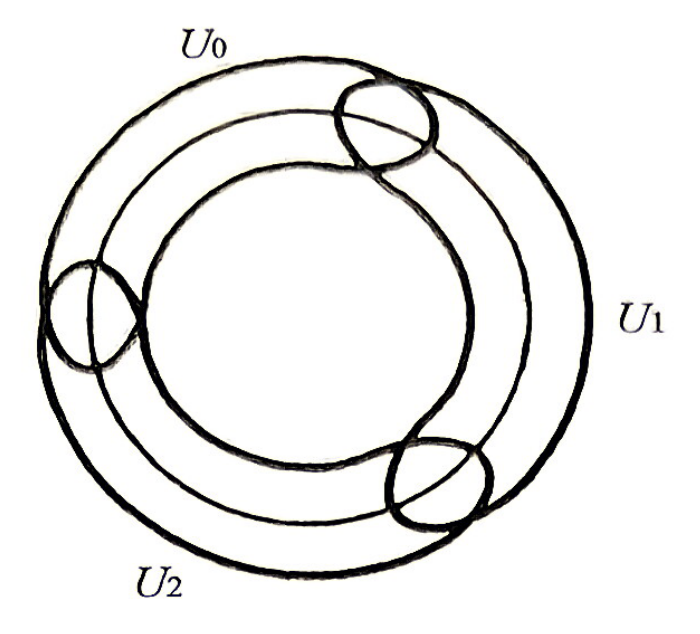
\includegraphics[width=0.48\linewidth]{figures/fig_p310_1.png}
  \caption*{图 10.4\quad $S^1$ 的一个无环覆盖（原书 p.302, Figure 10.4；
  PDF p.310）}
\end{figure}

回忆：经典的（奇异）上同调群 $H^*(X;\mathbf k)$ 度量拓扑空间 $X$ 的复杂度。对层上
同调群可以问同样的问题。

\begin{wque}{10.3.1}
对层上同调而言，层上同调群度量的是什么——是拓扑空间 $X$ 的复杂度，还是层
$\mathcal F$ 的复杂度？
\end{wque}

为回答这个问题，我们需要从更高级的视角来看待层上同调理论，这一视角称为\textbf{导出
函子}（derived functor），将在下一节引入。

% [Tutor Note: 含糊点拨——问题 10.3.1 的答案要点：层上同调\emph{同时}依赖二者，但
% 它作为「导出函子 $R\Gamma(X,\cdot)$ 的第 $*$ 阶」只依赖于层 $\mathcal F$（在
% 导出范畴中）与空间 $X$ 的整体信息；当 $\mathcal F=\mathbf k_X$ 为常值层时，
% $H^*(X;\mathbf k_X)=H^*(X;\mathbf k)$ 退化为经典上同调。例 10.3.2 中
% $\mathcal F=\mathbf{k}_{(0,1]}$ 的 $H^0$ 消失，说明层自身的「支撑」也会影响上同调。
% 下一节的导出范畴语言会精确表述「取截面 $\Gamma$ 不正合」如何被 $R\Gamma$ 修正。]
